%% -*- coding: utf-8; -*-

\documentclass[master,american]{ThesisPUC}

%---------- Math ----------%
\usepackage{amsmath}
\usepackage{amssymb}
\usepackage{mathtools}
\usepackage{bbm}
%---------- Floting ----------%
\usepackage{float}
% ---------- References ----------%
%\usepackage[sort&compress,round,comma,numbers]{natbib}
%\usepackage{natbib}
\usepackage[square,sort,comma,numbers]{natbib}
\usepackage[capitalise]{cleveref}
%---------- Algorithm ----------%
\usepackage[algosection, algoruled]{algorithm2e}
%---------- Tables ----------%
\usepackage{multicol}
\usepackage{booktabs}
%---------- TiKz ----------%
\usepackage{threeparttable}
\usepackage{standalone}
\usepackage{xcolor,listings}
\usepackage{tikz}
\usepackage{psfrag,epsf}
\usepackage{todonotes}
\usepackage{multirow}

\graphicspath{{images/}}

% ---------- Cover ----------%
% Adjust the advisor's title according to gender(Prof. or Prof$^{\text{a}}$.)
\author{Alexandre Marangoni Costa}
\authorR{Costa, Alexandre Marangoni}
\advisor{Marcus Vinicius Soledade Poggi de Aragão}{Prof.}
\advisorR{Poggi de Aragão, Marcus V.S.}
%\coadvisor{Simone Diniz Junqueira Barbosa}{Prof$^{\text{a}}$.}
%\coadvisorR{Barbosa, Simone Diniz Junqueira}

% This thesis will use colored figures, this goes in the catalographic sheet
\usecolour{true}
\title{Visão teórica e prática sobre a aplicação de Deep Learning na construção de agentes de pôquer}
\titleuk{Deep learning overview and application to build poker playing agents}

\day{26$^{th}$}
\month{February}
\myyear{2019}

% CDD is the registry number of the area, given by the library. Our area (informatics) is 004.
\city{Rio de Janeiro}
\CDD{004}
\department{Informática}
\program{Informática}
\school{Centro Técnico Científico}
\university{Pontifícia Universidade Católica do Rio de Janeiro}
\uni{PUC-Rio}

%---------- Jury ----------%

% Internal jury members are declared with \jurymember{name}{title}{department}{university}
% external jury members are declared with \extjurymember{name}{title}{university}
\jury{
  \jurymember{Hélio Côrtes Vieira Lopes}{Prof.}{Departamento de Informática}{PUC-Rio}
  \jurymember{Thibaut Vidal}{Prof.}{Departamento de Informática}{PUC-Rio}
  \jurymember{Bruno Feijó}{Prof.}{Departamento de Informática}{PUC-Rio}
  % The person below is mandatory.
  \schoolhead{Márcio da Silveira Carvalho}{Prof.}
}

%---------- Front letters ----------%
\resume
{
Bachelor's in Computer Engineer (2013) at the Pontifícia Universidade Católica do Rio de Janeiro (PUC-Rio). Joined the Master Program in Informatics at the Pontifical Catholic University of Rio de Janeiro (PUC-Rio) in 2017.
}

\acknowledgment
{
  \noindent
  
  To FAPERJ and CAPES, for financing this research.
  
  To Marcus Poggi, who is an advisor but also a close friend.
  
  To my family, for unconditional love.
  
  To my friends, who turn life into a beautiful journey.
  
  To Alan Turing, for making computation a reality.
  
  To God, for making everything a reality.
}


% Workaround for keywords. The keywords in the catalographic sheet must be separated by dots, while the ones shown in the abstract must be separated by semi-colons.
% Thats why we have two commands for each language: \keywords declares the keywords for the catalographic sheet, while \keywordsabstract declares the ones for the abstract.
\keywords
{
  \key{Deep Learning}
  \key{Redes Neurais}
  \key{Aprendizado de Máquina}
  \key{Pôquer}
  \key{Simulação Multiagente}
}

\keywordsabstract
{
  \key{Deep Learning;}
  \key{Redes Neurais;}
  \key{Aprendizado de Máquina;}
  \key{Pôquer;}
  \key{Simulação Multiagente;}
}

\keywordsuk
{
  \key{Deep Learning}
  \key{Neural Network}
  \key{Machine Learning}
  \key{Poker}
  \key{Multi-Agent Simulation}
}

\keywordsabstractuk
{
  \key{Deep Learning;}
  \key{Neural Network;}
  \key{Machine Learning;}
  \key{Poker;}
  \key{Multi-Agent Simulation;}
}

\abstract{
  A ciência de dados precisa de uma grande quantidade de dados para testar e melhorar soluções. Jogos são largamente usados para abstrair situações da vida real. Rodadas de pôquer são um bom exemplo pois, por não saber as cartas dos oponentes, o jogador analisa um cenário de informação incompleta numa competição de agentes que envolve conhecimento probabilístico, análise de risco e brefe. Isso o diferencia de xadrez, damas e jogos de conhecimento perfeito e algoritmos de busca em forca bruta sobre o espaço de soluções. Usar o pôquer como um caso de teste possibilita a análise de diferentes abordagens usadas na vida real, porém num cenário mais controlado. Esta dissertação propõe um arcabouço de funcionalidades para criar e testar diferentes algorítimos de Deep Learning, que podem jogar pôquer entre sí, aprender com o histórico e maximizar suas recompensas.
}

\abstractuk{
  Data science research needs real examples to test and improve solutions. Games are widely used to mimic those real-world examples. Poker rounds are a good example of imperfect information state with competing agents dealing with probabilistic knowledge, risk assessment, and possible deception, unlike chess, checkers and perfect information brute-force search style of games. By using poker as a test-bed we can analyze different approaches used in real-world examples, in a more controlled environment, which should give great insights on how to tackle those real-world scenarios. We propose a framework to build and test different neural networks that can play against each other, learn from a supervised experience and maximize its rewards.
}

\epigraph{"Hard" is everything you still don't know}
\epigraphauthor{Hamazaki, Geiza}

% WARNING
% The epigraph, if present, must come before the first chapter, always.
% There is a list of abreviations (abrevs.tex) which is included automatically in the ThesisPUC.cls, and is optional, comment the %% -*- coding: utf-8; -*-

\begin{thenotations}

  \noindent
  \begin{tabular}{ll}
    ANP -- Agência Nacional do Petróleo\\
    CENPES -- Centro de Pesquisas Leopoldo Américo Miguez de Mello\\
    LAMP -- Local Affine Multidimensional Projection\\
    MDS -- Multidimensional Scaling\\
    MP -- Multidimensional Projections\\
    $N_p$ -- Cumulative oil production\\
    P$_{10}$ -- Percentile $10$\\
    P$_{50}$ -- Percentile $50$\\
    P$_{90}$ -- Percentile $90$\\
    PETROBRAS -- Petróleo Brasileiro S.A.\\
    $Q_o$ -- Oil flow\\
    $Q_w$ -- Water flow\\
    $W_p$ -- Cumulative water production\\
  \end{tabular}

\end{thenotations} line if you do not wish to included it.
\begin{document}

%%% -*- coding: utf-8 -*-
\newpage

\chapter{Introduction}
\label{chap:introduction}

\section{Motivations}
\label{sec:motivations}
Different games were historically used to benchmark and explore Artificial Intelligence algorithms. In the last twenty years, several games like Chess, Checkers, Go, Backgammon and even Atari games were solved~\cite{Kocsis2006}, with algorithms reaching strategies that could win from professional players. To solve these style of games, a player has to take a decision given a perfect information scenario. In other words, all the information concerning the game state is available to the player: board configuration in case of board games, screen state in case of Atari games. Since there is no hidden information about the game, a brute-force search can retrieve the best action~\cite{Billings1998} with confidence.

But real life is not like that. According to von Neumann, founder of modern game theory, “real life consists of bluffing, of little tactics of deception, of asking yourself what is the other man going to think I mean to do. And that is what games are about in my theory.”~\cite{Bronowski1973}

In poker, a player’s private cards give asymmetric information about the state of the game. Each player sees a different state of the game, and none of them sees the complete state. This is why poker is called an Imperfect Information game and why it's hard to model and solve. Even if a better strategy is played, it can lose from a worse strategy because it has better cards, or it has bluffed or even changed strategy. To give a perspective, an example of an incomplete information board game is Battleship, while Chess is a perfect information game.

Along with that, the number of possible states in Heads-Up No-Limit Texas Hold’em Poker is approximately $10^{160}$ . Heads-Up means there are only two players in the table, so the number of states in a multiplayer table is even bigger. In comparison, chess and backgammon have $10^{47}$ and $10^{20}$ game states respectively~\cite{Johanson2013}. The universe has approximately $10^{80}$ atoms.

Limit Texas Hold’em Poker, a game variation in which players can only raise bets to a fixed amount, have around $10^{13}$ decision points in a heads-up game, and for that, it is a lot easier to solve a Limit poker variant. In fact, it was solved in 2015 by the Cepheus algorithm, developed by the Computer Poker Research Group at University of Alberta, and a joint effort with Oskari Tammelin, a Finnish software developer~\cite{Tammelin2015}.

Furthermore, card games have an element of chance when the deck is shuffled, before dealing the cards. Also, in Texas Hold'em early rounds (named pre-flop, flop, and turn) players have to act before seeing all dealt cards. A player's chance might change when a public card is revealed. This is why poker is classified as a stochastic game, in other words, not deterministic. An example of a stochastic board game is Backgammon, while Chess and Checkers are examples of deterministic games.

Real-world problems, like network and airport security, financial and energy trading, traffic control, routing, business negotiations and forecasting (weather, politics, etc) involve decision making with imperfect information and high-dimensional information states with a huge number of decision points ~\cite{Silver2016}, like poker. Those problems have some characteristics that require intelligent behavior~\cite{Billings1998}. We can map many of those characteristics to poker aspects:

\vspace{0.5cm}
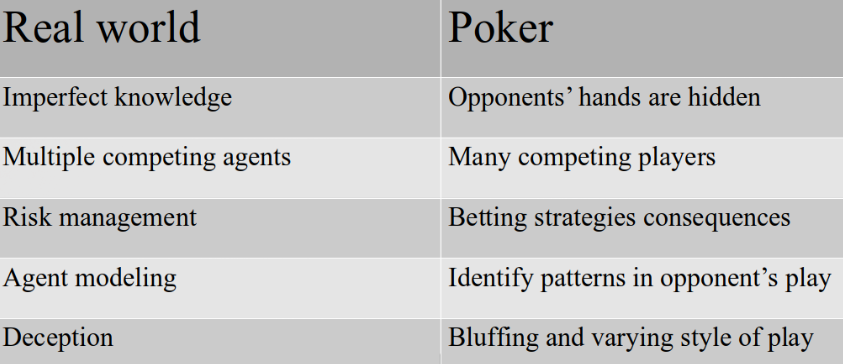
\includegraphics[scale=0.4]{real-world}
\vspace{0.5cm}

An optimal solution to these problems would be a Nash equilibrium, a strategy that if an agent deviates, it loses. If it follows, it wins. If an opponent also follows, both tie. Simple machine learning methods achieve near-optimal solutions to perfect information games but fail to converge in imperfect information games. Using a controlled environment such as poker, allows one to measure progress in a domain where simple machine learning does not converge to near-optimal solutions.

\section{Goals}
\label{sec:goals}

The imperfect information property, the stochastic property, along with the size of the game makes solving of multiplayer No-Limit Texas Hold’em Poker an interesting milestone for Computer Science, not reached until now. This work proposes Pucker, a framework to help scientists reach this goal, providing a consistent simulation of the game, storage of past scenarios in an efficient way, a learning  and prediction strategy for machine learning algorithms, and some examples of algorithms to help the development of better strategies.

The best Pucker agent is inspired by reinforcement learning, similar to David Silver's work ~\cite{Silver2016}, but adds domain knowledge and state abstraction to learn multiplayer No Limit Texas Hold'em. In the end, we show how to measure progress and display a consistent evaluation of the agent's incremental learning.

Unfortunately, there are several caveats in learning from a generated dataset. A learning model requires a fine representation of poker state, with information such as private and public cards, previous opponents' actions, and any known public information the enables a gradient descent model to approach incremental learning. Also, the training data obtained from simulation of deterministic weak players are not sophisticated enough to generate a model competitive against serious players.

To deal with these challenges, we propose a high dimensional representation composed with most of the information used by professional players, along with statistical features built by simulation of future rounds, that improved early stage poker actions such as flop actions. Also, we improved the dataset by running multiple phases of learning, whereas the first phase relies on data generated by deterministic players, and further phases learn from data generated from deep learning sophisticated players. Finally, we propose a method inspired by genetic algorithms, to prevent reaching a local best response by generating populations of algorithms from the most winners. In the end, we acknowledge that the last descendants of this population are capable of better actions.

In summary,  our contributions are:

\begin{itemize}
  \item A framework to build Texas Hold'em agents;
  \item A simulation of the game that can be used to generate input dataset in an efficient way;
  \item Several deterministic players used to generate initial data and measure learning progress;
  \item A state representation that players can use to learn best actions;
  \item A learning and prediction neural network that leverages reinforcement learning to learn a multi-step game such as poker;
\end{itemize}


\section{Dissertation Structure}
\label{sec:organization}

The remainder of this thesis is organized as follows:

\begin{itemize}
  \item Chapter~\ref{chap:background} we describe \textbf{how to play poker} and the \textbf{related work};
  \item Chapter~\ref{chap:learning} shows how \textbf{neural networks} work to gradually improve its predictions and how we used reinforcement learning to adapt the model to multi-step games;
  \item Chapter~\ref{chap:architecture} describes the project \textbf{architecture}, simulation, data storage, learn and predict modules;
  \item Chapter~\ref{chap:evaluation} presents the experiments and the associated \textbf{results};
  \item Chapter~\ref{chap:conclusions} presents some \textbf{concluding remarks} and directions for the future work;
\end{itemize}

%%% Local Variables:
%%% mode: latex
%%% TeX-master: thesis.tex
%%% End:

%%% -*- coding: utf-8 -*-
\newpage

\chapter{Background}
\label{chap:background}

\section{Poker Foundations}
\label{sec:foundations}

Texas Hold'em poker variant starts with every player receiving 2 private cards. Then, there is a betting round: every player bets some amount that they have the best hand. This first round is called \textbf{pre-flop}.

Next, 3 public cards are dealt to the table. This is called \textbf{flop}. The flop is public, and those 3 cards are shared among all players. A betting round happens again, but now the players bet who has the best combination of private hand and shared table, a total of 5 cards. Every bet goes to the table pot.

Afterward, there is the \textbf{turn} round. A card is dealt to the table, followed by a betting round. Finally, another card is dealt to the table - the \textbf{river} round - and the last betting round finishes the game.

A player with the best combination of private and public cards wins the pot. Also, a player wins if all other players have given up. In case of tie, winners share the table pot.
 
The bet can be a fold, a call of the previous bet or a raise. When a player folds, he is out of this game and loses the amount he has previously given to the table pot. Each player announces it's bet starting from the first player after the dealer until every player but one fold or every active player bet the same amount (call). 

\vspace{2cm}
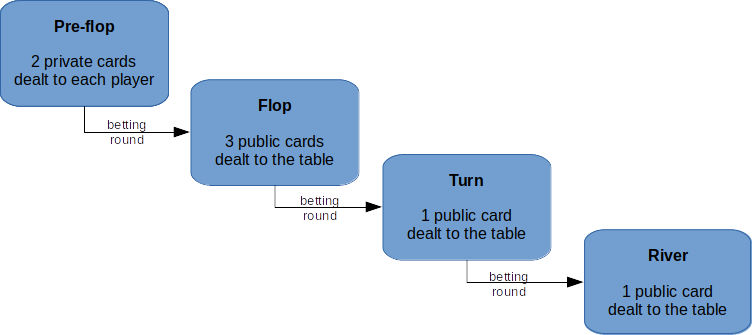
\includegraphics[scale=2]{poker-foundations}
\vspace{0.5cm}

\subsection{Hand Ranking}

The hands are listed bellow in ranking order:

High card: all five cards of different rank and a variety of suits;

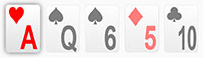
\includegraphics[scale=2]{high-card}

One pair: two cards of the same rank and three different cards;
  
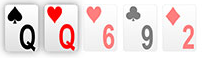
\includegraphics[scale=2]{pair}

Two pairs: two pairs and one different card;

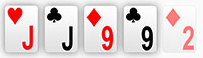
\includegraphics[scale=2]{two-pairs}
  
Three of a kind: three cards of the same rank and two different cards;
  
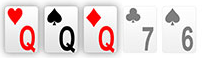
\includegraphics[scale=2]{three-of-a-kind}

Straight: five cards in sequence of rank with different suits;
  
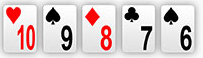
\includegraphics[scale=2]{straight}
  
Flush: five cards of the same suit;
  
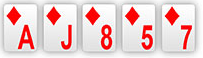
\includegraphics[scale=2]{flush}
  
Full House: three cards of the same rank and two cards of the same rank;
  
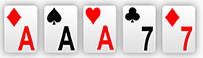
\includegraphics[scale=2]{full-house}
  
Four of a kind: four cards of the same rank;
  
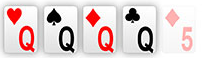
\includegraphics[scale=2]{four-of-a-kind}
  
Straight flush: a straight of the same rank;
  
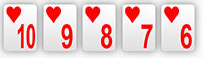
\includegraphics[scale=2]{straight-flush}
 
If two players have the same type of hand, the hand with higher card wins. A player can use a combination of its private cards and the public cards in the table. In the end, a player has 7 cards available but can combine only 5 in a poker hand.

\subsection{Positions}
\label{sec:positions}

It is trivial to understand that player's position matters. The last player to bet have more information about other players' bets and can take a better decision in order to maximize its rewards.

In each round, each player is the \textbf{dealer} of the deck, in sequence. The player next to the dealer is the \textbf{small-blind} and the next player is the \textbf{big-blind}. In pre-flop, the small-blind have to place a minimum bet and the big-blind has to place twice the small-blind. To participate, every player has to bet as least the big-blind amount. In the next round, the flop, bets start from zero.

In this work, we will consider a game of 5 players, therefore, there will be 5 positions, and each player will be dealer, small-blind, and big-blind, once every 5 games.

\subsection{Actions}

Given a state of the game, a player can

\begin{itemize}
  \item \textbf{Bet}: to place an amount to the pot when no one has done it before
  \item \textbf{Raise}: to raise a previous bet
  \item \textbf{Call}: to bet the same amount of a previous bet
  \item \textbf{Fold}: to give up, and lose the money placed in the pot
  \item \textbf{Check}: when no bet has been made, a player can pass (it's the same as betting an amount of 0)
\end{itemize}

Also, in no-limit poker a player can bet all of its money. This is called \textbf{all-in}

\subsection{Variants}
Poker variants usually differ in orthogonal dimensions. The two most common are number of players and betting structure.

A \textbf{heads-up} variant includes two players. The \textbf{ring} variant includes more than two players and we will refer to it as multiplayer variant. This work concerns about multiplayer poker but can be extended to the heads-up variant.

In the \textbf{limit} variant, also called \textit{fixed limit}, the players can only raise to a fixed amount, usually the big-blind amount or twice the big-blind. In \textbf{no-limit} poker, a raise can be anything from the last bet to the players total stack.

\section{Related Work}
\label{chap:related-work}

The first computer program to play poker was called Orac, and was created by Mike Caro to compete in World Series of Poker in 1984.

Afterward, University of Alberta, Carnegie Mellon and University of Auckland led the development of poker bots.

In 1998, the Computer Poker Research Group at University of Alberta, led by Michael Bowling, released Loki, an artificial intelligence capable of playing Limit Heads-Up Texas Hold’em ~\cite{Billings2016}. Next, they improved their work and created Poki, in 2000 ~\cite{Davidson2000}. Both of them focused in modeling the opponent’s strategy, but still relied in “search” by simulation to find the best decision.

In 2003, scientists began to shift from the chess methodology model, and in 2008 a poker bot developed in University of Alberta, called Polaris, played 6 heads up No Limit Hold’em matches against humans, with 3 wins, 2 losses and 1 tie.

Next, in 2009, University of Auckland introduced Sartres, its first poker AI. It was designed to play specifically heads up Limit Texas Hold’em, and was the first one to use a case-based reasoning methodology ~\cite{Rubin2009}.

Counterfactual Regret Minimization started to play a big whole in this field ~\cite{Zikenvich2008}, and Limit Texas Hold’em was essentially solved in 2015, by Cepheus, another AI developed at the Computer Poker Research Group at University of Alberta ~\cite{Bowling2008}.

Also in 2015, a professor at Carnegie Mellon University developed Claudico ~\cite{Brown2015}, a No Limit Texas Hold’em bot, but it lost heads up matches against pro players. It required  a Pittsburgh supercomputer with 16 terabytes of RAM to learn the its strategy.

Libratus succeeded Claudico, but was rewritten from scratch. It was build with more than 15 million core hours of computation, compared to 3 million performed for Claudico. It applied a new variant of Counterfactual Regret Minimization, namely CFR+, developed by Oskari Tammelin, a scientist involved in the Cepheus project ~\cite{Brown2017}.

In 2016 David Silver introduced Neural Fictitious Self Play, a deep reinforcement learning method composed of two neural networks that learn approximate Nash equilibria of imperfect-information games. Silver's goal was to not rely on engineering abstractions or any domain knowledge, and still be capable of learning in a complex environment. It was applied to Limit Texas Hold'em and approached the performance of state-of-the-art~\cite{Silver2016}.

Finally, in 2017 the Computer Research Group (UoA) together with several scientists from the Czech Republic, introduced DeepStack, an algorithm for imperfect information scenarios. This work combined many different deep learning strategies, like recursive reasoning, to handle information asymmetry, decomposition to focus computation on the relevant decision, and a form of intuition algorithm to automatically learn from self-play ~\cite{Moravcik2017}. For the first time, a computer program defeated with statistical significance professional poker players in heads-up no-limit Texas Hold’em.

%%% Local Variables:
%%% mode: latex
%%% TeX-master: thesis.tex
%%% End:

%%% -*- coding: utf-8 -*-
\newpage

\chapter{Learning}
\label{chap:learning}

\section{Deep Learning}
\label{sec:deep-learning}

Deep Learning is a branch of machine learning responsible for studying complex architectures, with the pourpose of learning patterns in data representations. The \textit{deep} in the name refers to the depth of layers in the architectures, as it can be very deep.

Most of the models in Deep Learning are composed of Artificial Neural Networks. Those neural networks were first proposed by McCulloch and Pitts~\cite{McCulloch1943}, in 1943, and were inspired by the processing and communication patterns in biological nervous systems, although there are many differences and even more from human brains. Those differences make the study of Artificial Neural Networks incompatible with the study of neuroscience.

\subsection{The perceptron}
The first ANN model was implemented by Frank Rosenblatt~\cite{Rosenblatt1958}, and was called \textit{the perceptron}. The perceptron was composed of multiple inputs, an output, a collection of weights and an activation function. It was capable of learning binary classification by supervised learning.

\begin{center}
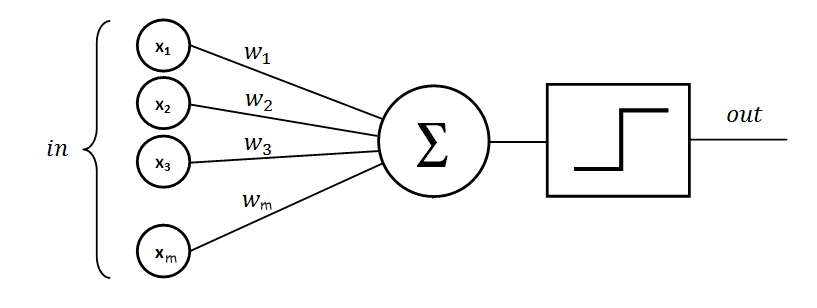
\includegraphics[width=1\columnwidth]{perceptron}
\end{center}

Mathmatically, the perceptron is a function that maps the input $\boldsymbol{x}$ to a binary output $\boldsymbol{f(x)}$.

\begin{minipage}{\textwidth}
\begin{center}
$
f(x)=\begin{cases}
1 & \text{ if } \boldsymbol{w \cdot x} + b > 0 \\
0 & \text{ otherwise }
\end{cases}
$
\end{center}

\vspace{0.5cm}

\hspace{4.5cm}$\boldsymbol{w \cdot x}$ is the dot product $\sum_{i=1}^{m}w_{i}x_{i}$,

\hspace{4.5cm}$w$ is a vector of weights

\hspace{4.5cm}$m$ is the number of inputs

\hspace{4.5cm}$b$ is the bias
\end{minipage}

\vspace{0.5cm}

This model was heavily criticized because it couldn't learn a simple XOR function, as it can only simulate linearly separable functions. To overcome this, Rumelhart, Hinton and Willians~\cite{Rumelhart1986} proposed the Backpropagation algorithm, which implemented another layer and finally was capable of simulating non-linearity.

Nowadays, Artificial Neural Networks are composed of multiple neurons, and multiple layers of neurons. Each neuron works similar to a perceptron.

\subsection{Activation Functions}

As the name sugests, the activation functions are responsible for setting the activation of a neuron, in other words, it sets how the input signal is passed to the output.

The first activation function, proposed by McCulloch and Pitts, was the threshold fuction. This function is binary, it is equals to 1 (passes the signal) if the input signal is greater than 0, and it does not passes the signal otherwise, as in above perceptron description.

Another common activation function is the sigmoid. Unlike the threshold function, the sigmoid function is smoother, and can be mathmatically described as $\phi(x) = 1/(1+e^{-x})$. This function is usually used in the last layer of classification models to describe the probability of the signal being 0 or 1, and that's where the smoothness is helpfull instead of the binary threshold.

Then, there is the rectifier function $\phi(x) = max(0, x)$. Nowadays, it is one of the most popular functions for Artificial Neural Networks, thanks to the work of Glorot, Bordes and Bengio, who proved it allowed faster and better training of ANNs~\cite{Glorot2010}.

Finally, there is the hyperbolic tangent function, which is similar to the sigmoid function, but it goes from 1 to -1. The sigmoid function can "stuck" the training of ANNs, because when a strongly-negative input is provided, the sigmoid function outputs values very near to zero, inactivating the neuron instead of passing a negative signal~\cite{Glorot2010.2}. Thus, the hyperbolic tangent function is usually preferable. Mathmatically, it can be described as $\phi(x) = (1-e^{-2x})/(1+e^{-2x})$.

\vspace{0.5cm}

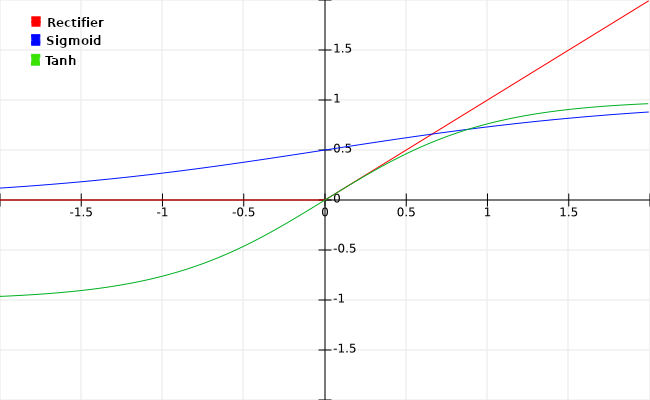
\includegraphics[width=1\columnwidth]{activation-functions}



\section{Reinforcement Learning}
\label{sec:reinforcement-learning}

%%% Local Variables:
%%% mode: latex
%%% TeX-master: thesis.tex
%%% End:

%%% -*- coding: utf-8 -*-
\newpage

\chapter{Architecture}
\label{chap:architecture}

The Pucker framework has 4 components: a no limit Texas Hold’em simulation written in JRuby~\cite{jruby.org}, a SQLite storage~\cite{sqlite.org}, a learning and a prediction script written in Python programming language~\cite{python.org}.

The simulation runs the game, inserting data about the states seen by a player and his rewards (or punishments if negative) in the database. The states and rewards are the learning variables. The learning script reads the database, fits the model, and stores the model parameters in disk. The prediction script loads the model and exposes predictions through an HTTP API. The simulation queries the prediction API when a machine learning player needs to take a decision.

\vspace{1cm}
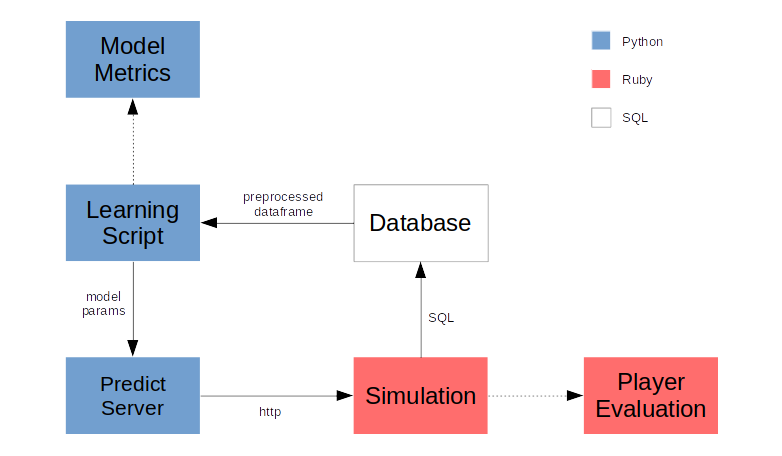
\includegraphics[scale=2]{architecture}

\section{Simulation}
\label{sec:simulation}

The Ruby programming language was chosen to write the simulation component. Ruby offers a great syntax to write game simulations because it is idiomatic, succinct, and object-oriented.

The game of poker, as many other games, is composed of independent reusable components that answer to messages, such as player, dealer and a deck of cards. According to Ampatzoglou and Chatzigeorgiou~\cite{Ampatzoglou2007}, games demand great flexibility, code reusability and low maintenance costs. Consequently, the application of design patterns in them can be beneficial. Ruby is heavily object-oriented and allowed fast development of the simulation.

Due to its idiomacy, the main method of the simulation, the \textit{play} method on the \textit{Game} class, can be understood by anyone. It seems like an english description of the poker game:

\begin{lstlisting}[
    float=h,
    caption=game.rb,
    language=Ruby,
    basicstyle=\tiny\ttfamily,
    commentstyle = \color{gray},
    keywordstyle=\color{red},
    stringstyle=\color{blue},
]
def play
  setup_game
  collect_blinds

  # FLOP
  3.times { deal_table_card }
  bets = collect_bets
  main_pot.merge!(bets)

  # TURN
  deal_table_card
  bets = collect_bets
  main_pot.merge!(bets)

  # RIVER
  deal_table_card
  bets = collect_bets
  main_pot.merge!(bets)

  winners = eligible_players_by_rank
  reward winners

  rotate_and_reset_states
end
\end{lstlisting}

A simple random player can be written in few lines of ruby:

\begin{lstlisting}[
    float=h,
    caption=game.rb,
    language=Ruby,
    basicstyle=\tiny\ttfamily,
    commentstyle = \color{gray},
    keywordstyle=\color{red},
    stringstyle=\color{blue},
]
class DummyPlayer < Player
  def bet(state)
    min_bet = state.min_bet

    choice = rand

    if min_bet > 0 && choice < 1/3.0 # FOLD
      fold
    elsif choice < 2/3.0 # CHECK
      get_from_stack(min_bet)
    else # RAISE
      raise_from(min_bet)
    end
  end
end
\end{lstlisting}

Through the past years, many reusable poker components were written by the Computer Poker Research Group, at the University of Alberta ~\cite{spaz.ca/poker/doc}. Those components were written in the Java programming language. To reuse those components, we chose the JRuby platform to run the poker simulation. This platform runs the Ruby syntax on the Java Virtual Machine~\cite{jruby.org}, and simplifies the calling of Java poker components from Ruby simulation code.

In the context of the Pucker framework, a game has a group of players, a dealer and a pot with the bets of the current game. The dealer deal cards. Players evaluate game state and choose an action based on their current state.

\vspace{1cm}
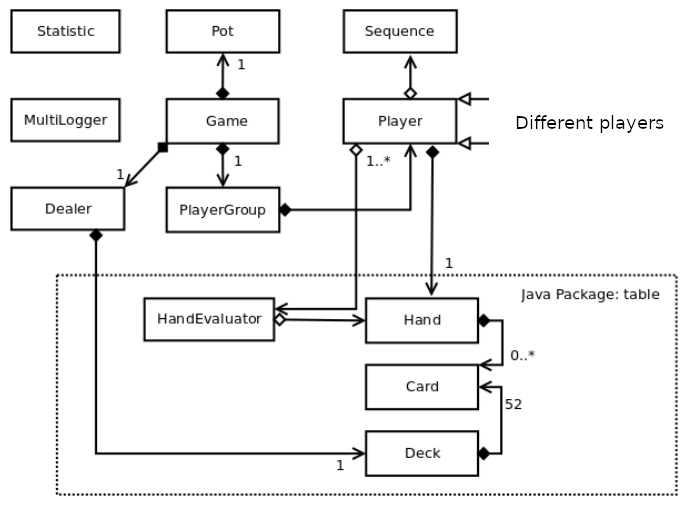
\includegraphics[scale=2]{simulation-diagram}

As previously said (see~\ref{sec:foundations}), Texas Hold'em poker variant has 4 phases: pre-flop, flop, turn and river.

In pre-flop, a player have to take an action with little information about its opponents, since few bets have been committed to the pot. Given that, in pre-flop a player must deal with more imperfect information than in further rounds of the game. Due to its complexity, this research have abstracted the pre-flop phase: every player bets the same as the big-blind player (see~\ref{sec:positions}).

\section{Storage}
\label{sec:storage}

In real poker, there are many game variables, such as how much time a player delayed to take a decision, history of opponent’s decisions, cards on the table, cards in player’s private hand, how strong is the combination of table and hand cards, player position, and many others.

In Pucker, we consider a state as composed by:
\begin{itemize}
  \item Count of players
  \item Count of active players in this round (players who have not folded)
  \item Player's position
  \item Amount in the pot
  \item Amount each player has bet
  \item Number of raises per player
  \item Self amount committed to the pot
  \item Self number of raises
  \item Hand cards
  \item Table cards
  \item Combination of Hand and Table ranking
  \item Combination of Hand and Table strength
  \item Combination of Hand and Table potential
  \item Action taken
\end{itemize}

The reward (or punishment if negative) a player has received in the end of a round is also part of the state. This is the dependent variable our models are trying to predict. Pucker is an extensible framework, it is easy to add or remove variables to the state in future work.

In poker, a player sees a game state, takes an action, and receives a reward (or punishment) in the end of the round. Pucker players remember the states, actions and rewards, and stores them in a SQLite database, one row per action taken.

This is a complex game. To learn a fine strategy, a machine learning player must be fitted from a very large dataset. To accomplish that, the simulation needs to be fast and can't be stopped every round by a slow operation such as database inserts. To overcome this problem, a batch of states are written at once in a single insert query.

\section{Learning}
\label{sec:Learning}

A machine learning prediction typically maps a set of variables to an output. In this work, the input will be the poker state and the output will be the reward seen in the end of this state. In short, the machine learning algorithm will learn to predict the reward, given a state and an action.

To choose the right action, a machine learning player will predict the reward of different actions (fold, call, raise), and choose an action that maximises its rewards. This is inspired in Reinforcement Learning, but without policy optimization~\cite{Silver2016}.

Since the number of states in no limit Texas Hold’em is $10^{160}$~\cite{Johanson2013}, it is impossible to store every state. It is even hard to store the number of states to take a good decision. To overcome this, we will store only the model parameters and erase the database of states after the learning process.

It is crucial for the model to be extensible: it may correct its parameters according to new data, it will not be able to access the full history. Neural Networks are naturally capable of incremental learning, and this is a big reason of their choice in favor of other models, like Gradient Boosting Machines. According to~\cite{xgboost-github}, until today popular Gradient Boosting Machine implementations cannot handle inclemental learning.

Instead of considering the game round (pre-flop, flop, turn or river) a variable of the state, past work~\cite{Sirin2008} and ~\cite{Moravcik2017} has seen better results by creating a separate model for different rounds, and we will also consider that. The main reason is that different rounds of poker are played in very different ways because they have a different state. Additionally, the number of possible states in poker is huge~\cite{Johanson2013}, by using different models in different rounds we are reducing the number of possible states a model has to learn from.

The learning component is a Python script that reads states from a database, preprocess, fits a prediction model and stores its parameters in disk.

\subsection{Neural Networks Architectures}

\subsection{Bayesian Networks and Initial Dataset}
\label{sec:data-generation}

In order to train a supervised model, it is needed a dataset. The performance of a machine learning model relies heavily on the quality of this dataset~\cite{Polikar2001}. A realiable dataset must represent reality with confidence, thus it should be generated from real situations.

In Pucker, after the models are trained, new datasets can be generated from subsequential games played by those models. But still remains the problem of how to generate a initial dataset with good quality.

Untrained Neural Networks could be put to play. Since their parameters are not fitted yet, they will play randomly according to the random generation of its initial parameters. The quality of this dataset is worse than a dataset generated from good players, because it represents random situations, hardly seen in professional games.

Pucker Framework introduces a initial set of simple players that are put to play against each other. Rather than playing randomly, those players use Bayesian Networks~\cite{Heckerman1998} to analyse state and choose better poker actions. To certify that Bayesian players perform better, they were put to play against random players and won by a large margin in the long run. They were also tested against "always check" players, and won by a large margin.

Bayesian networks are tree structures that represent conditional dependencies of variables in a directed acyclic graph, and are capable of infere from those variables~\cite{Neapolitan2003}.

Nodes of this graph represents Bayesian variables. In poker, those nodes can represent the poker state: hand ranking, number of players, position, etc. Unconnected nodes represent variables that are conditionally independent of each other, like a player hand and position. Nodes are associated with a probability function that represents the chance of possible states of that node. Edges represent conditional dependencies, for example, a good poker hand depends on the private player hand and the public table cards.

After some experiments, two different architectures were chosen to compose poker players in order to generate a initial dataset. The first one in simpler, and relies only on the state minimum bet and hand rank. The second uses players' position, together with minimum bet, to compose a scenario conditional variable. When the Bayesian Network detects a high winning condition, bayesian players raise. When it detects a low winning condition, bayesian players check. If it's a losing condition, it folds, or checks if minimum bet is zero.

As an example, the bayesian player represented by figure~\ref{fig:simple-bn} will fold with a bad hand when there is a minimum bet over zero. And it will re-raise when it has a great hand and the minimum bet is over zero.

\begin{figure}[H]
  \centering
  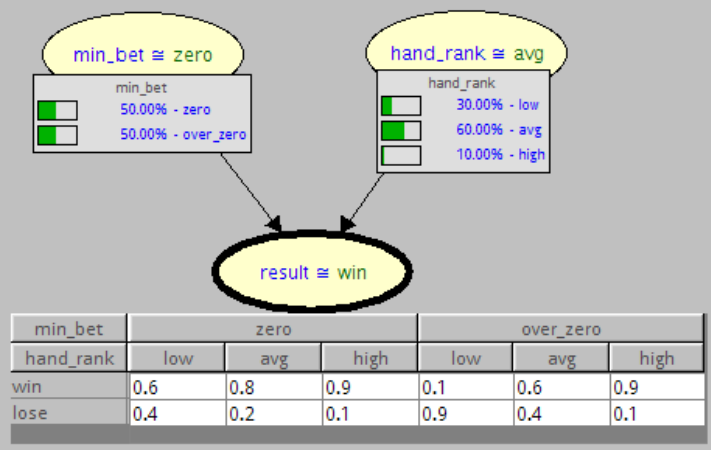
\includegraphics[width=1\textwidth]{simple_bn}
  \caption{Simple bayesian network with its probabilities}
  \label{fig:simple-bn}
\end{figure}

\begin{figure}[H]
  \centering
  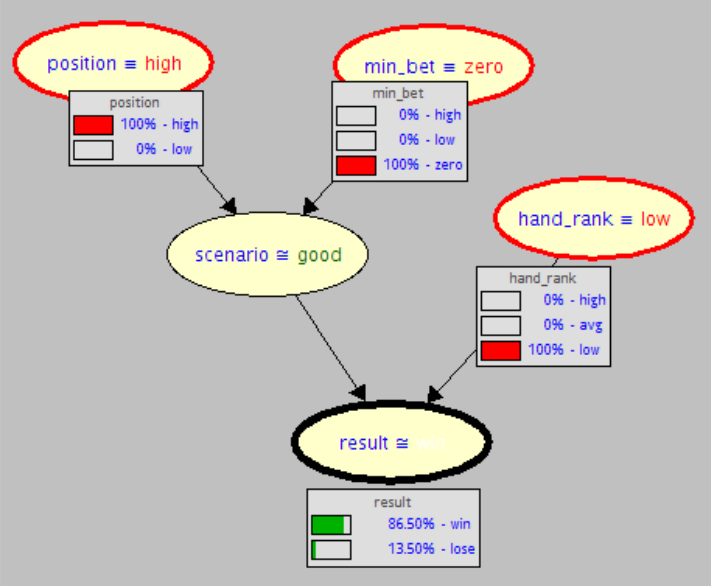
\includegraphics[width=1\textwidth]{best_bn}
  \caption{Better bayesian network. It is represented a situation of high position, zero bets and low hand rank. This player might bluff in this situation.}
\end{figure}
\vspace{0.5cm}

Those two bayesian networks played 40000 games in a five players Texas Hold'em table. This table also had a random player to generate diverse situations in order to generalize the initial dataset. The result is a 566739 row database that was used to train the initial neural networks. After that, the neural networks played against each other, generated even better quality datasets, and learned incrementally from their self-plays.


\section{Prediction}
\label{sec:prediction}

The prediction component is trivial. It reads the stored model parameters and creates an instance of the model ready to predict from new states.

There are two problems: this is a slow process, and the Ruby simulation cannot run Python code seamlessly, as they are different languages running in different virtual machines. To overcome those problems, the prediction component keeps an instance of the model in memory and exposes an HTTP API that receives a state and returns a prediction.

This component is capable of exposing many different models, one per HTTP endpoint. This way, Pucker supports the simulation of many different machine learning algorithms playing at the same time.

To build the HTTP API, Pucker uses the Flask library~\cite{flask.pocoo.org}.

%%% Local Variables:
%%% mode: latex
%%% TeX-master: thesis.tex
%%% End:

%%% -*- coding: utf-8 -*-
\newpage

\chapter{Evaluation}
\label{chap:evaluation}

\section{Model metrics}
\label{sec:metrics}

\section{Poker statistics}
\label{sec:statistics}


%%% Local Variables:
%%% mode: latex
%%% TeX-master: thesis.tex
%%% End:

%% -*- coding: utf-8 -*-
\newpage

\chapter{Conclusions}
\label{chap:conclusions}

This chapter presents the concluding remarks about our work. Discuss our contributions in Section~\ref{sec:contributions}, and present directions for future works in Section~\ref{sec:future-work}.

In this thesis, we presented a novel graphical approach to scenario reduction on time series ensembles. We evaluated the feasibility of our proposal by performing an empirical study with a series of potential users, both experienced in the area and not. By observing their interactions and interviewing them afterwards, we obtained valuable insights on the usefulness of our proposal. Following from the results of our previous publication we have expanded our work in two aspects: (i)~use glyph sizes to represent the time in the Time-lapsed LAMP chart; (ii)~in the same chart, encode the uncertainty inherent to the data. The first expansion was done in order to fix an issue related to the abstraction created by employing multidimensional-projections using time-varying data. The second expansion aims to help users to quickly identify time ranges with high variance in the data.

Besides the user study, we also compared our results with other approaches in the literature and industry. proposes to select a set of representative scenarios under different well configurations. Their approach handles several simulation parameters and responses simultaneously, thus, selecting representative scenarios based on multiple criteria. The Industry approach selects scenarios with cumulative production closest to the target references at the end of the simulation. Both approaches are well suited depending on the post-processing tasks and the data itself. In our tests, our approach selected scenarios with consistently smaller error when compared to both the Industry and Clustering approaches. It must be stated, however, that this does not mean that our approach is better, only that it yields good scenarios when the objective function is the proximity to a reference in a context where the scenarios' evolution must be taken into consideration.


\section{Publications}
\label{sec:publications}

\section{Contributions}
\label{sec:contributions}

\section{Future Work}
\label{sec:future-work}


The remainder of this thesis is organized as follows: Chapter~\ref{chap:related-work} presents the state-of-the-art in Artificial Intelligent poker agents. Next, in Chapter~\ref{chap:background} we describe poker foundations and explain computer poker features that can help convergence of neural networks in early poker stages. Chapter~\ref{chap:learning} shows how neural networks work to gradually improve its predictions and how we used reinforcement learning to adapt the model to multi-step games. Chapter~\ref{chap:architecture} describes the project architecture, simulation, data storage, learn and predict modules. Chapter~\ref{chap:evaluation} presents details about the experiments and the associated results. Chapter~\ref{chap:conclusions} presents some concluding remarks and directions for future work.

\arial
\bibliography{references}

% Apendix chapters below.
%\normalfont
%\appendix
%\newpage

\chapter{User profile questionnaire for prototype evaluation sessions}
\label{chap:profile-form}

\begin{enumerate}
\item Personal information
  \begin{enumerate}
 \item Name
 \newline \rule[0pt]{300pt}{1pt}
 \item E-mail
 \newline \rule[0pt]{300pt}{1pt}
 \item Education degree
 \newline \rule[0pt]{300pt}{1pt}
 \item Course semester (just for students)
 \newline \rule[0pt]{300pt}{1pt}
 \item Occupation
 \newline \rule[0pt]{300pt}{1pt}
  \end{enumerate}
\item Please mark below your knowledge about the following subjects:
	\begin{enumerate}
   \item Division of a sample by percentiles: P10, P50, P80 ...
		\newline \circle{10} I do not know
     \newline \circle{10} I know little (I have learned these concepts at some point, but may have to learn again if I have to apply them)
     \newline \circle{10} I have average knowledge (I may have to revise one concept or another if I have to apply it)
     \newline \circle{10} I know well (I do not apply often, but I would not need to revise the concepts if I had to apply them)
     \newline \circle{10} I am a specialist (I apply these concepts frequently)
	  \newline 
   \item Analysis of trends and patterns in time series
   \newline \circle{10} I do not know
   \newline \circle{10} I know little (I have learned these concepts at some point, but may have to learn again if I have to apply them)
   \newline \circle{10} I have average knowledge (I may have to revise one concept or another if I have to apply it)
   \newline \circle{10} I know well (I do not apply often, but I would not need to revise the concepts if I had to apply them)
   \newline \circle{10} I am a specialist (I apply these concepts frequently)\\
      
   \item Projection chart (Time-lapsed LAMP chart)
   \begin{figure}[H]
		\centering
		\includegraphics[width=0.9\columnwidth]{images/form-timelapsedchart.png}
		\label{fig:form-timelapsedchart}
	   \end{figure}

   \circle{10} I do not know
   \newline \circle{10} I know little (I have learned these concepts at some point, but may have to learn again if I have to apply them)
   \newline \circle{10} I have average knowledge (I may have to revise one concept or another if I have to apply it)
   \newline \circle{10} I know well (I do not apply often, but I would not need to revise the concepts if I had to apply them)
   \newline \circle{10} I am a specialist (I apply these concepts frequently)\\

 \newpage
       \item Ranking chart (Bump chart)
       \begin{figure}[H]
 		\centering
 		\includegraphics[width=0.9\columnwidth]{images/form-bumpchart.png}
 		\label{fig:form-bumpchart}
 	   \end{figure}
       
       \circle{10} I do not know
       \newline \circle{10} I know little (I have learned these concepts at some point, but may have to learn again if I have to apply them)
       \newline \circle{10} I have average knowledge (I may have to revise one concept or another if I have to apply it)
       \newline \circle{10} I know well (I do not apply often, but I would not need to revise the concepts if I had to apply them)
       \newline \circle{10} I am a specialist (I apply these concepts frequently)\\

 \newpage
       \item Distance chart
       \begin{figure}[H]
 		\centering
 		\includegraphics[width=0.9\columnwidth]{images/form-distancechart.png}
 		\label{fig:form-distancechart}
 	   \end{figure}
      
       \circle{10} I do not know
       \newline \circle{10} I know little (I have learned these concepts at some point, but may have to learn again if I have to apply them)
       \newline \circle{10} I have average knowledge (I may have to revise one concept or another if I have to apply it)
       \newline \circle{10} I know well (I do not apply often, but I would not need to revise the concepts if I had to apply them)
       \newline \circle{10} I am a specialist (I apply these concepts frequently)\\

 \newpage
       \item Fanchart
       \begin{figure}[H]
 		\centering
 		\includegraphics[width=0.9\columnwidth]{images/form-fanchart.png}
 		\label{fig:form-fanchart}
 	  \end{figure}
      
       \circle{10} I do not know
       \newline \circle{10} I know little (I have learned these concepts at some point, but may have to learn again if I have to apply them)
       \newline \circle{10} I have average knowledge (I may have to revise one concept or another if I have to apply it)
       \newline \circle{10} I know well (I do not apply often, but I would not need to revise the concepts if I had to apply them)
       \newline \circle{10} I am a specialist (I apply these concepts frequently)

     \end{enumerate}
\end{enumerate}

\end{document}
